\documentclass{beamer}
%
% Choose how your presentation looks.
%
% For more themes, color themes and font themes, see:
% http://deic.uab.es/~iblanes/beamer_gallery/index_by_theme.html
%
\mode<presentation>
{
  \usetheme{default}      % or try Darmstadt, Madrid, Warsaw, ...
  \usecolortheme{default} % or try albatross, beaver, crane, ...
  \usefonttheme{default}  % or try serif, structurebold, ...
  \setbeamertemplate{navigation symbols}{}
  \setbeamertemplate{caption}[numbered]
} 

\usepackage[english]{babel}
\usepackage[utf8x]{inputenc}
\usepackage{multirow}
\usepackage{booktabs}
\usepackage{bigstrut}
\usepackage{hyperref}


\begin{document}




\begin{frame}{Datasets}

\begin{table}[]
    \centering
    \begin{tabular}{cccc}
    \toprule  
    Datasets & Users & Items & Ratings\\
    \midrule  
    Instant Video & 426922 & 23965 & 583933  \\
    Musical Instrument & 339231 & 83046 & 500176  \\
    Video Games & 826767 & 50210 & 1324753  \\
    \bottomrule
    \end{tabular}
    \caption{Statistics of the datasets}
\end{table}

\subsection{Evaluation methods}
    
    
\end{frame}










\begin{frame}{Datasets}


\begin{figure}
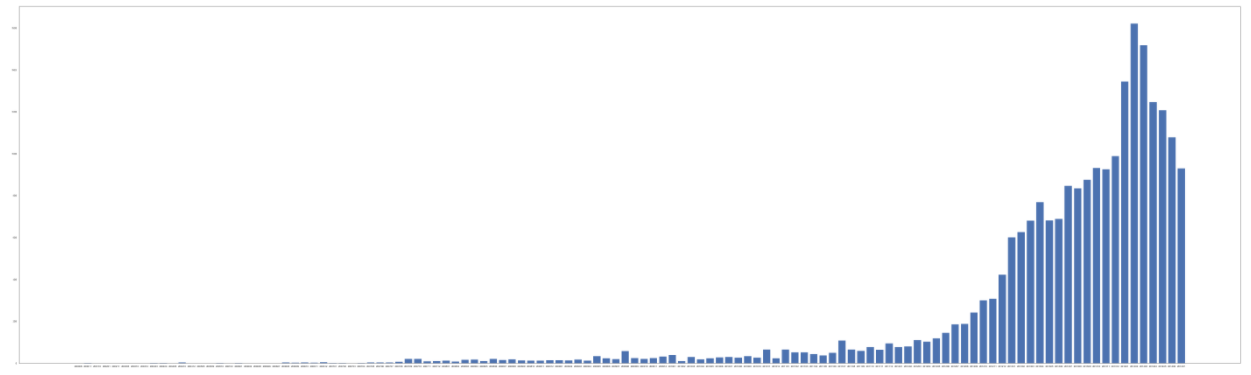
\includegraphics[height=3cm]{figure1.png}
\caption{Ratings of Instant Video ordered in time}
\end{figure}


\end{frame}










\begin{frame}{Datasets}


\begin{figure}
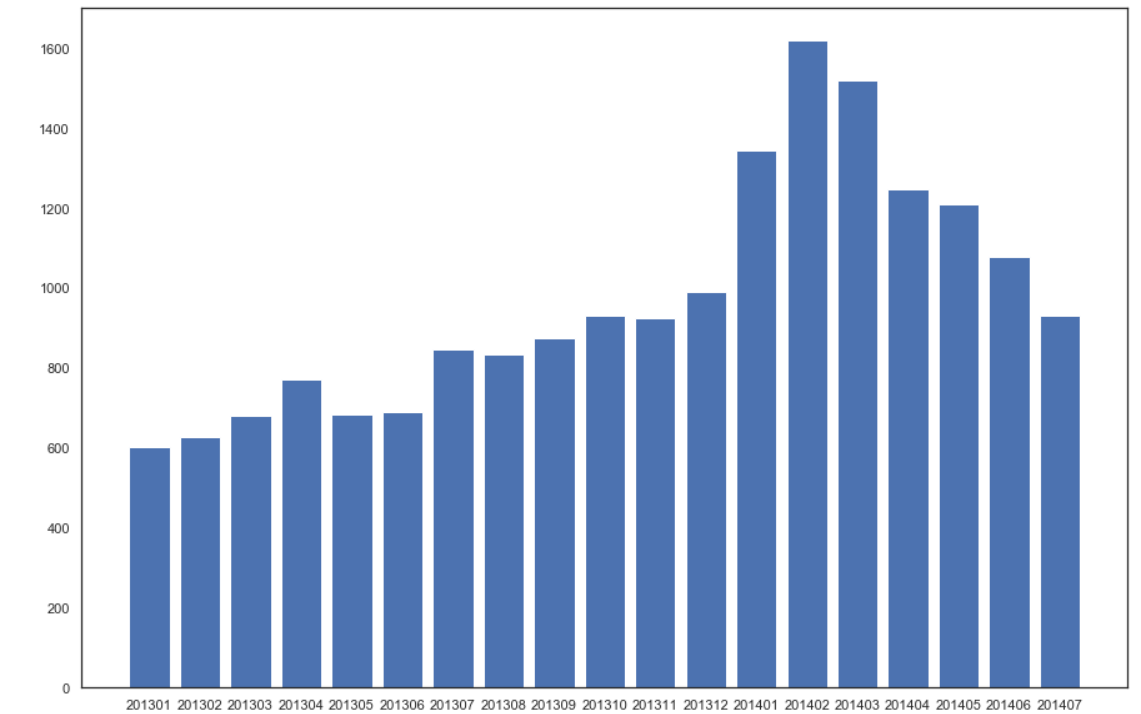
\includegraphics[height=5cm]{figure2.png}
\caption{Ratings of Instant Video ordered in time}
\end{figure}


\end{frame}










\begin{frame}{Datasets}

\begin{table}[]
    \centering
    \begin{tabular}{cccc}
    \toprule  
    Datasets & Users & Items & Ratings\\
    \midrule  
    Instant Video & 426922 & 23965 & 583933  \\
    Musical Instrument & 339231 & 83046 & 500176  \\
    Video Games & 826767 & 50210 & 1324753  \\
    \bottomrule
    \end{tabular}
    \caption{Statistics of the raw datasets}
\end{table}


\begin{table}[]
    \centering
    \begin{tabular}{cccc}
    \toprule  
    Datasets & Users & Items & Ratings\\
    \midrule  
    Instant Video & 688 & 3288 & 6717 \\
    Musical Instrument & 1408 & 5771 & 7906 \\
    Video Games & 1003 & 5297 & 10472  \\
    \bottomrule
    \end{tabular}
    \caption{Statistics of the preprocessed datasets}
\end{table}
    
    
\end{frame}









\begin{frame}{Evaluation}


\begin{table}[htbp]
  \centering
  \setlength{\tabcolsep}{1mm}{
    \begin{tabular}{c|ccc|ccc|ccc}
    \hline
    Datasets & \multicolumn{3}{c|}{Instant Video} & \multicolumn{3}{c|}{Musical Instruments} & \multicolumn{3}{c}{Video Games} \\
    \hline
    \hline
    Measures@10(\%) & P     & R     & F1    & P     & R     & F1    & P     & R     & F1 \\
    \hline
    SVD   & 0.59 & 3.21 & 0.97 & 0.10 & 0.31 & 0.14 & 0.28 & 1.30 & 0.45 \\
    kNN   & 0.40 & 2.04 & 0.66 & 0.14 & 1.09 & 0.24 & 0.40 & 1.76 & 0.64 \\
    BPR   & 0.68 & 3.61 & 1.11 & 0.23 & 1.57 & 0.39 & 0.75 & 3.30 & 1.20 \\
    SLIM  & 1.39 & 6.98 & 2.25 & 0.17 & 1.10 & 0.29 & 1.02 & 4.11 & 1.59 \\
    \hline
    \hline
    \end{tabular}%
  \label{tab:addlabel}%
  \caption{The performance of baselines}
  }
\end{table}%

\end{frame}

\end{document}
